%%%%%%%%%%%%%%%%%%%%%%%%%%%%%%%%%%%%%%%%%
% Classicthesis Typographic Thesis
% LaTeX Template
% Version 1.1 (4/8/12)
%
% This template has been downloaded from:
% http://www.LaTeXTemplates.com
%
% Original author:
% André Miede (http://www.miede.de)
%
% License:
% CC BY-NC-SA 3.0 (http://creativecommons.org/licenses/by-nc-sa/3.0/)
%
% General Tips:
% 1) Make sure to edit the classicthesis-config.file
% 2) New enumeration (A., B., C., etc in small caps): \begin{aenumerate} \end{aenumerate}
% 3) For margin notes: \marginpar or \graffito{}
% 4) Do not use bold fonts in this style, it is designed around them
% 5) Use tables as in the examples
% 6) See classicthesis-preamble.sty for useful commands
%
%%%%%%%%%%%%%%%%%%%%%%%%%%%%%%%%%%%%%%%%%

%----------------------------------------------------------------------------------------
%	PACKAGES AND OTHER DOCUMENT CONFIGURATIONS
%----------------------------------------------------------------------------------------

\documentclass[
		twoside,openright,titlepage,numbers=noenddot,headinclude,%1headlines,
                footinclude=true,cleardoublepage=empty,
                BCOR=5mm,paper=a4,fontsize=11pt, % Binding correction, paper type and font size
                english, % Languages
                ]{scrreprt} 
                
% Includes the file which contains all the document configurations and packages - make sure to edit this file
%%%%%%%%%%%%%%%%%%%%%%%%%%%%%%%%%%%%%%%%%
% Thesis Configuration File
%
% The main lines to change in this file are in the DOCUMENT VARIABLES
% section, the rest of the file is for advanced configuration.
%
%%%%%%%%%%%%%%%%%%%%%%%%%%%%%%%%%%%%%%%%%

%----------------------------------------------------------------------------------------
%	DOCUMENT VARIABLES
%	Fill in the lines below to enter your information into the thesis template
%	Each of the commands can be cited anywhere in the thesis
%----------------------------------------------------------------------------------------

% Remove drafting to get rid of the '[ Date - classicthesis version 4.0 ]' text at the bottom of every page
\PassOptionsToPackage{eulerchapternumbers,listings,pdfspacing,subfig,beramono,eulermath,parts,dottedtoc,tocaligned}{classicthesis}
% Available options: drafting parts nochapters linedheaders eulerchapternumbers beramono eulermath pdfspacing minionprospacing tocaligned dottedtoc manychapters listings floatperchapter subfig
% Adding 'dottedtoc' will make page numbers in the table of contents flushed right with dots leading to them

\newcommand{\myTitle}{Photogrammetrie-Evaluation\xspace}
\newcommand{\mySubtitle}{xspace}
\newcommand{\myReportName}{Technical Report Nr. 1501}
\newcommand{\myName}{Danilo Bargen, Josua Schmid\xspace}
\newcommand{\myProf}{Prof. Stefan Keller\xspace}
\newcommand{\myUni}{HSR Hochschule fuer Technik Rapperswil\xspace}
\newcommand{\myFaculty}{IFS Institut fuer Software / Geometa Lab\xspace}
\newcommand{\myHackerspace}{Coredump Rapperswil\xspace}
\newcommand{\myLocation}{Rapperswil, Schweiz\xspace}
\newcommand{\myTime}{Fruehling 2015\xspace}
\newcommand{\myVersion}{version 1.0\xspace}
\newcommand{\myLicense}{CC BY-SA 3.0 Switzerland\xspace}
\newcommand{\myKeywords}{3D Printing, CAD, Cross Compilers, Data Analysis, Data
Visualization, OpenSCAD, Python, Software Libraries, Statistics, Tangible}
\newcommand{\myRepo}{\url{https://github.com/coredump-ch/photogrammetry-evaluation/}\xspace}

%----------------------------------------------------------------------------------------
%	USEFUL COMMANDS
%----------------------------------------------------------------------------------------

\newcommand{\ie}{i.\,e.}
\newcommand{\Ie}{I.\,e.}
\newcommand{\eg}{e.\,g.}
\newcommand{\Eg}{E.\,g.} 
\newcommand{\zb}{z.\,B.} 

\newcommand{\tangible}{\emph{Tangible}}

\newcounter{dummy} % Necessary for correct hyperlinks (to index, bib, etc.)
\providecommand{\mLyX}{L\kern-.1667em\lower.25em\hbox{Y}\kern-.125emX\@}

%----------------------------------------------------------------------------------------
%	PACKAGES
%----------------------------------------------------------------------------------------

\usepackage{lipsum} % Used for inserting dummy 'Lorem ipsum' text into the template

%------------------------------------------------
 
\PassOptionsToPackage{utf8}{inputenc}
\usepackage{inputenc}
 
%------------------------------------------------

\PassOptionsToPackage{ngerman}{babel}
\usepackage{babel}

%------------------------------------------------			

\PassOptionsToPackage{square,numbers}{natbib}
\usepackage{natbib}
 
%------------------------------------------------

\PassOptionsToPackage{fleqn}{amsmath} % Math environments and more by the AMS 
\usepackage{amsmath}
 
%------------------------------------------------

\PassOptionsToPackage{T1}{fontenc}
\usepackage{fontenc}

%------------------------------------------------

\usepackage{xspace} % To get the spacing after macros right

%------------------------------------------------

\usepackage{mparhack} % To get marginpar right

%------------------------------------------------

\usepackage{fixltx2e} % Fixes some LaTeX stuff 

%------------------------------------------------

\PassOptionsToPackage{smaller}{acronym} % Include printonlyused in the first bracket to only show acronyms used in the text
\usepackage{acronym} % nice macros for handling all acronyms in the thesis

%------------------------------------------------

%\renewcommand*{\acsfont}[1]{\textssc{#1}} % For MinionPro
%\renewcommand{\bflabel}[1]{{#1}\hfill} % Fix the list of acronyms

%------------------------------------------------

\PassOptionsToPackage{pdftex}{graphicx}
\usepackage{graphicx} 
\usepackage{subfig}

%------------------------------------------------

\usepackage{pgf} 
\usepackage{tikz} 
\usepackage{tikz-qtree}
\usetikzlibrary{}

%------------------------------------------------

\usepackage{wrapfig}

%------------------------------------------------

\usepackage{siunitx}

%------------------------------------------------

\PassOptionsToPackage{shortcuts}{extdash}
\usepackage{extdash}

%------------------------------------------------

\usepackage{rotating}

%------------------------------------------------

\usepackage{needspace}

%------------------------------------------------

\newcommand{\ja}{Ja}
\newcommand{\nein}{Nein}


%----------------------------------------------------------------------------------------
%	FLOATS: TABLES, FIGURES AND CAPTIONS SETUP
%----------------------------------------------------------------------------------------

\usepackage{tabularx} % Better tables
\setlength{\extrarowheight}{3pt} % Increase table row height
\newcommand{\tableheadline}[1]{\multicolumn{1}{c}{\spacedlowsmallcaps{#1}}}
\newcommand{\myfloatalign}{\centering} % To be used with each float for alignment
\usepackage{caption}
\captionsetup{format=hang,font=small}
\usepackage{subfig}  

%----------------------------------------------------------------------------------------
%	CODE LISTINGS SETUP
%----------------------------------------------------------------------------------------

\usepackage{minted} % Syntax highlighting                                                                                                                                                                                                      
\usemintedstyle{tango}
\definecolor{tango-bg}{HTML}{F8F8F8}
\expandafter\def\csname PY@tok@err\endcsname{}

\newminted{python}{bgcolor=tango-bg,frame=lines,framesep=2mm,samepage=true,fontsize=\footnotesize}

%\usepackage{listings} 
%\lstset{emph={trueIndex,root},emphstyle=\color{BlueViolet}}%\underbar} % for special keywords
%\lstset{language=Python, % Specify the language for listings here
%keywordstyle=\color{RoyalBlue}, % Add \bfseries for bold
%basicstyle=\small\ttfamily, % Makes listings a smaller font size and a different font
%%identifierstyle=\color{NavyBlue}, % Color of text inside brackets
%commentstyle=\color{Green}\ttfamily, % Color of comments
%stringstyle=\rmfamily, % Font type to use for strings
%numbers=left, % Change left to none to remove line numbers
%numberstyle=\scriptsize, % Font size of the line numbers
%stepnumber=5, % Increment of line numbers
%numbersep=8pt, % Distance of line numbers from code listing
%showstringspaces=false, % Sets whether spaces in strings should appear underlined
%breaklines=true, % Force the code to stay in the confines of the listing box
%%frameround=ftff, % Uncomment for rounded frame
%frame=single, % Frame border - none/leftline/topline/bottomline/lines/single/shadowbox/L
%belowcaptionskip=.75\baselineskip % Space after the "Listing #: Desciption" text and the listing box
%}

%----------------------------------------------------------------------------------------
%	HYPERREFERENCES
%----------------------------------------------------------------------------------------

\PassOptionsToPackage{pdftex,hyperfootnotes=false,pdfpagelabels}{hyperref}
\usepackage{hyperref}  % backref linktocpage pagebackref
\pdfcompresslevel=9
\pdfadjustspacing=1

\hypersetup{
% Uncomment the line below to remove all links (to references, figures, tables, etc)
%draft, 
colorlinks=true, linktocpage=true, pdfstartpage=1, pdfstartview=FitV,
% Uncomment the line below if you want to have black links (e.g. for printing black and white)
%colorlinks=false, linktocpage=false, pdfborder={0 0 0}, pdfstartpage=1, pdfstartview=FitV, 
breaklinks=true, pdfpagemode=UseNone, pageanchor=true, pdfpagemode=UseOutlines,
plainpages=false, bookmarksnumbered, bookmarksopen=true, bookmarksopenlevel=1,
hypertexnames=true, pdfhighlight=/O, urlcolor=webbrown, linkcolor=RoyalBlue, citecolor=webgreen,
%------------------------------------------------
% PDF file meta-information
pdftitle={\myTitle},
pdfauthor={\textcopyright\ \myName, \myUni, \myFaculty},
pdfsubject={\mySubtitle},
pdfkeywords={\myKeywords},
pdfcreator={pdfLaTeX},
pdfproducer={LaTeX with hyperref and classicthesis}
%------------------------------------------------
}   

%----------------------------------------------------------------------------------------
%	BACKREFERENCES
%----------------------------------------------------------------------------------------

\usepackage{ifthen} % Allows the user of the \ifthenelse command
\newboolean{enable-backrefs} % Variable to enable backrefs in the bibliography
\setboolean{enable-backrefs}{false} % Variable value: true or false

\newcommand{\backrefnotcitedstring}{\relax} % (Not cited.)
\newcommand{\backrefcitedsinglestring}[1]{(Cited on page~#1.)}
\newcommand{\backrefcitedmultistring}[1]{(Cited on pages~#1.)}
\ifthenelse{\boolean{enable-backrefs}} % If backrefs were enabled
{
\PassOptionsToPackage{hyperpageref}{backref}
\usepackage{backref} % to be loaded after hyperref package 
\renewcommand{\backreftwosep}{ and~} % separate 2 pages
\renewcommand{\backreflastsep}{, and~} % separate last of longer list
\renewcommand*{\backref}[1]{}  % disable standard
\renewcommand*{\backrefalt}[4]{% detailed backref
\ifcase #1 
\backrefnotcitedstring
\or
\backrefcitedsinglestring{#2}
\else
\backrefcitedmultistring{#2}
\fi}
}{\relax} 

%----------------------------------------------------------------------------------------
%	AUTOREFERENCES SETUP
%	Redefines how references in text are prefaced for different 
%	languages (e.g. "Section 1.2" or "section 1.2")
%----------------------------------------------------------------------------------------

\makeatletter
\@ifpackageloaded{babel}
{
\addto\extrasamerican{
\renewcommand*{\figureautorefname}{Figure}
\renewcommand*{\tableautorefname}{Table}
\renewcommand*{\partautorefname}{Part}
\renewcommand*{\chapterautorefname}{Chapter}
\renewcommand*{\sectionautorefname}{Section}
\renewcommand*{\subsectionautorefname}{Section}
\renewcommand*{\subsubsectionautorefname}{Section}
}
\addto\extrasngerman{
\renewcommand*{\paragraphautorefname}{Absatz}
\renewcommand*{\subparagraphautorefname}{Unterabsatz}
\renewcommand*{\footnoteautorefname}{Fu\"snote}
\renewcommand*{\FancyVerbLineautorefname}{Zeile}
\renewcommand*{\theoremautorefname}{Theorem}
\renewcommand*{\appendixautorefname}{Anhang}
\renewcommand*{\equationautorefname}{Gleichung}
\renewcommand*{\itemautorefname}{Punkt}
}
\providecommand{\subfigureautorefname}{\figureautorefname} % Fix to getting autorefs for subfigures right
}{\relax}
\makeatother

%----------------------------------------------------------------------------------------

\usepackage{classicthesis} 

%----------------------------------------------------------------------------------------
%	CHANGING TEXT AREA 
%----------------------------------------------------------------------------------------

%\linespread{1.05} % a bit more for Palatino
%\areaset[current]{312pt}{761pt} % 686 (factor 2.2) + 33 head + 42 head \the\footskip
%\setlength{\marginparwidth}{7em}%
%\setlength{\marginparsep}{2em}%

%----------------------------------------------------------------------------------------
%	USING DIFFERENT FONTS
%----------------------------------------------------------------------------------------

%\usepackage[oldstylenums]{kpfonts} % oldstyle notextcomp
%\usepackage[osf]{libertine}
%\usepackage{hfoldsty} % Computer Modern with osf
%\usepackage[light,condensed,math]{iwona}
%\renewcommand{\sfdefault}{iwona}
%\usepackage{lmodern} % <-- no osf support :-(
%\usepackage[urw-garamond]{mathdesign} <-- no osf support :-(

%----------------------------------------------------------------------------------------
%	HYPHENATION
%----------------------------------------------------------------------------------------

\hyphenation{GoPro}
\hyphenation{Mesh-Lab}


\begin{document}

\frenchspacing % Reduces space after periods to make text more compact

\raggedbottom % Makes all pages the height of the text on that page

\selectlanguage{ngerman} % Select your default language - e.g. american or ngerman

%\renewcommand*{\bibname}{new name} % Uncomment to change the name of the bibliography
%\setbibpreamble{} % Uncomment to include a preamble to the bibliography - some text before the reference list starts

\pagenumbering{roman} % Roman page numbering prior to the start of the thesis content (i, ii, iii, etc)

\pagestyle{plain} % Suppress headers for the pre-content pages

%----------------------------------------------------------------------------------------
%	PRE-CONTENT THESIS PAGES
%----------------------------------------------------------------------------------------

% Title Page

\begin{titlepage}

\begin{addmargin}[-1cm]{-3cm}
\begin{center}
\large

\hfill
\vfill

\begingroup
\color{Maroon}{\LARGE\spacedallcaps{\myTitle}}\\ \bigskip % Thesis title
\endgroup

\spacedlowsmallcaps{\myName} \\
\spacedlowsmallcaps{\myHackerspace}

\vfill

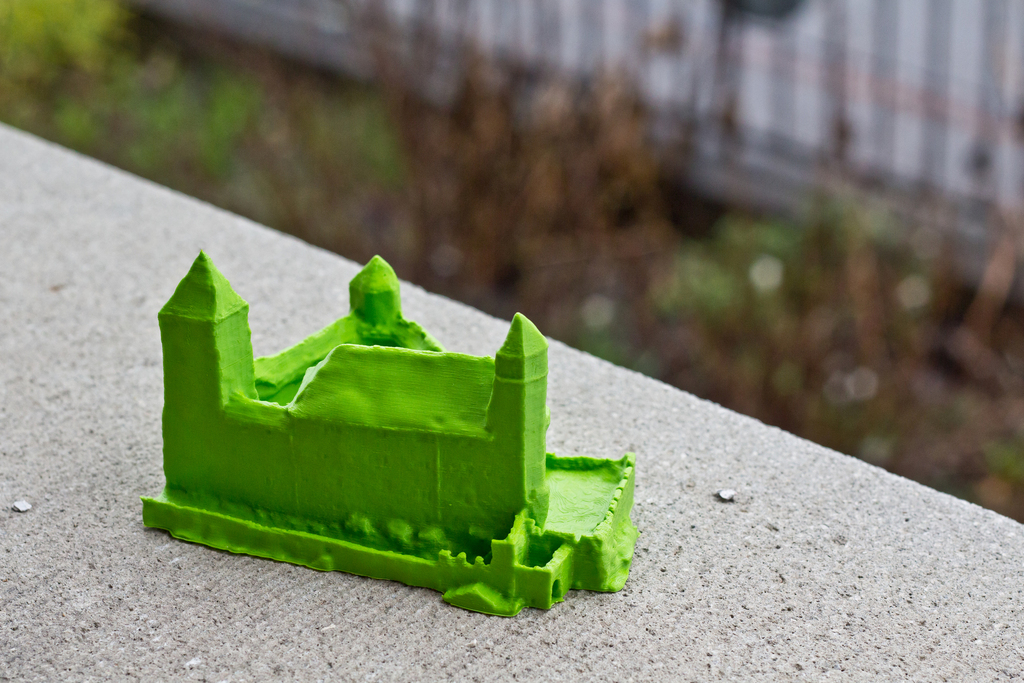
\includegraphics[width=13cm]{images/schloss} \\ \bigskip % Picture

\mySubtitle \\ % Thesis subtitle

\vspace{2cm}

Durchgeführt von \\
\vspace{4mm}
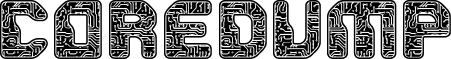
\includegraphics[width=6cm]{images/coredump-logo}

\vspace{10mm}

Im Auftrag von \\
\vspace{1mm}

\includegraphics[width=5cm]{images/HSR_Logo_CMYK}
\quad\quad

\includegraphics[width=4cm]{images/ifs-logo}


\end{center}
\end{addmargin}

\end{titlepage}
 % Main title page

% Back of the title page

\thispagestyle{empty}

\hfill

\vfill

\noindent\myName: \textit{\myTitle: 3D-Rekonstruktion Schloss Rapperswil und
Orthofoto-Erstellung HSR-Gelände mit Workflow, Software-Evaluation und
Dokumentation.}
\textcopyright\ \myTime

\bigskip

\noindent\spacedlowsmallcaps{Auftragnehmer}: \\
\myHackerspace

\medskip

\noindent\spacedlowsmallcaps{Projektpartnerin}: \\
\myUni \\
\myFaculty \\
\myProf

\medskip

\noindent\spacedlowsmallcaps{Ort}: \\
\myLocation

\medskip

\noindent\spacedlowsmallcaps{Zeitraum}: \\
\myTime

\medskip

\noindent\spacedlowsmallcaps{Lizenz}: \\
\myLicense

\medskip

\noindent\spacedlowsmallcaps{Dokumentations-URL}: \\
\myRepo

\medskip

\noindent\spacedlowsmallcaps{Kontakt}: \\
Danilo Bargen \texttt{<mail@dbrgn.ch>}\\
Josua Schmid \texttt{<jschmid@fastmail.net>}
 % Back of the title page

%\cleardoublepage\include{front_back_matter/dedication} % Dedication page

%\cleardoublepage\include{front_back_matter/foreword} % Uncomment and create a Foreword.tex to include a foreword

\cleardoublepage% Abstract

\pdfbookmark[1]{Abstract}{Abstract} % Bookmark name visible in a PDF viewer

\begingroup
\let\clearpage\relax
\let\cleardoublepage\relax
\let\cleardoublepage\relax

\chapter*{Abstract} % Abstract name

TODO

\endgroup			

\paragraph{Keywords:}\mbox{}\\
\textit{\myKeywords}

\vfill
 % Abstract page

\cleardoublepage% Acknowledgements

\pdfbookmark[1]{Acknowledgements}{Acknowledgements} % Bookmark name visible in a PDF viewer

\bigskip

%----------------------------------------------------------------------------------------

\begingroup

\let\clearpage\relax
\let\cleardoublepage\relax
\let\cleardoublepage\relax

\chapter*{Acknowledgements} % Acknowledgements section text

Wir möchten uns bei folgenden Personen bedanken:

\begin{itemize}
	\item Prof. Stefan Keller für die tatkräftige Unterstützung bei der
		Realisation dieses Projektes
	\item Michael Suter von lightmoment.ch für das Erstellen der
		Drohnen-Luftbilder (\autoref{workflow:drone})
	\item Jan Appenzeller von der Firma Drei-De für die Hilfe bei der
		Mesh-Nachbearbeitung (\autoref{workflow:mesh-cleanup})
	\item Der Ortsgemeinde Rapperswil-Jona für das Bereitstellen von Grundrissen
		des Schlosses
	\item Prof. Dr.-Ing. André Miede für das verwendete \emph{classicthesis}
		\LaTeX-Template
	\item TODO more?
\end{itemize}


\endgroup
 % Acknowledgements page

\pagestyle{scrheadings} % Show chapter titles as headings

\cleardoublepage% Table of Contents - List of Tables/Figures/Listings and Acronyms

\refstepcounter{dummy}

\pdfbookmark[1]{\contentsname}{tableofcontents} % Bookmark name visible in a PDF viewer

\setcounter{tocdepth}{2} % Depth of sections to include in the table of contents - currently up to subsections

\setcounter{secnumdepth}{3} % Depth of sections to number in the text itself - currently up to subsubsections

\manualmark
\markboth{\spacedlowsmallcaps{\contentsname}}{\spacedlowsmallcaps{\contentsname}}
\tableofcontents
\automark[section]{chapter}
\renewcommand{\chaptermark}[1]{\markboth{\spacedlowsmallcaps{#1}}{\spacedlowsmallcaps{#1}}}
\renewcommand{\sectionmark}[1]{\markright{\thesection\enspace\spacedlowsmallcaps{#1}}}

\clearpage

\begingroup
\let\clearpage\relax
\let\cleardoublepage\relax
\let\cleardoublepage\relax

%----------------------------------------------------------------------------------------
%	List of Figures
%----------------------------------------------------------------------------------------

\refstepcounter{dummy}
\addcontentsline{toc}{chapter}{\listfigurename} % Uncomment if you would like the list of figures to appear in the table of contents
%\pdfbookmark[1]{\listfigurename}{lof} % Bookmark name visible in a PDF viewer

\listoffigures

\vspace*{8ex}
\newpage

%----------------------------------------------------------------------------------------
%	List of Tables
%----------------------------------------------------------------------------------------

%\refstepcounter{dummy}
%\addcontentsline{toc}{chapter}{\listtablename} % Uncomment if you would like the list of tables to appear in the table of contents
%\pdfbookmark[1]{\listtablename}{lot} % Bookmark name visible in a PDF viewer
%
%\listoftables
%
%\vspace*{8ex}
%\newpage

%----------------------------------------------------------------------------------------
%	List of Listings
%----------------------------------------------------------------------------------------

%\refstepcounter{dummy}
%\addcontentsline{toc}{chapter}{\lstlistlistingname} % Uncomment if you would like the list of listings to appear in the table of contents
%\pdfbookmark[1]{\lstlistlistingname}{lol} % Bookmark name visible in a PDF viewer
%
%\lstlistoflistings
%
%\vspace*{8ex}
%\newpage

%----------------------------------------------------------------------------------------
%	Acronyms
%----------------------------------------------------------------------------------------

\refstepcounter{dummy}
\addcontentsline{toc}{chapter}{Glossar} % Uncomment if you would like the acronyms to appear in the table of contents
%\pdfbookmark[1]{Acronyms}{acronyms} % Bookmark name visible in a PDF viewer

\markboth{\spacedlowsmallcaps{Acronyms}}{\spacedlowsmallcaps{Acronyms}}

\chapter*{Glossar}

\begin{acronym}[UML]
	\acro{DOM / DSM}{Digitales Oberflächenmodell (engl. Digital Surface Model)}
	\acro{G-Code}{Code bestehend aus CNC Instruktionen, wird häufig für 3D-Drucker
	einesetzt.}
	\acro{GIS}{Geografische Informationssysteme}
	\acro{GNSS}{Global Navigation Satellite System, \zb{} GPS, GLONASS oder
	Galileo.}
	\acro{HSR}{Hochschule für Technik Rapperswil}
	\acro{Orthofoto}{Eine verzerrungsfreie und massstabsgetreue Abbildung der
	Erdoberfläche, die durch photogrammetrische Verfahren aus Luft- oder
	Satellitenbildern abgeleitet wird.}
	\acro{Photogrammetrie}{Eine Gruppe von Messmethoden und Auswerteverfahren der
	Fernerkundung, um aus Fotografien und genauen Messbildern eines Objektes seine
	räumliche Lage oder dreidimensionale Form zu bestimmen.}
	\acro{SFM}{Structure From Motion, eine Methode um 3D-Modelle aus "<bewegten
	Bildern"> zu erzeugen.}
	\acro{STL}{STereoLithography, ein für 3D-Druck geeignetes Dateiformat.}

\end{acronym}

\endgroup

\cleardoublepage
 % Contents, list of figures/tables/listings and acronyms

\pagenumbering{arabic} % Arabic page numbering for thesis content (1, 2, 3, etc)
%\setcounter{page}{90} % Uncomment to manually start the page counter at an arbitrary value (for example if you wish to count the pre-content pages in the page count)

\cleardoublepage % Avoids problems with pdfbookmark

%----------------------------------------------------------------------------------------
%	THESIS CONTENT - CHAPTERS
%----------------------------------------------------------------------------------------

\part{Einleitung}

\chapter{Einleitung}

\label{ch:einleitung}

%----------------------------------------------------------------------------------------

Dieses Kapitel erläutert kurz den Ursprung dieses Projektes sowie dessen Ziele.

%----------------------------------------------------------------------------------------

\section{Das Crowdfunding-Projekt}\label{sec:crowdfunding}

Wir sind Mitglieder des im Herbst 2013 in Rapperswil gegründeten Hackerspaces
"<Coredump">\footnote{\url{https://www.coredump.ch/}}. Unsere Ziele sind der
kreative Umgang mit Technologie sowie der Know-How Austausch an regelmässigen
Treffen. Wir möchten unseren Mitgliedern gute Infrastruktur für technische
Projekte, v.a. im Bereich der Informatik und Elektrotechnik bieten.

\marginpar{Die Schweizer Crowdfunding-Plattform wemakeit wurde im Februar 2012
von der Kulturkommunikatorin Rea Eggli, dem Künstler Johannes Gees und dem
Interaction Designer Jürg Lehni gegründet und ist mittlerweile die grösste
Crowdfunding-Plattform in der Schweiz.}

Um die Herstellung von selbst gestalteten 3D-Teilen zu ermöglichen, starteten
wir im Januar 2015 ein Crowdfunding-Kampagne auf
Wemakeit\footnote{\url{https://wemakeit.com/projects/3d-drucker-fuer-rapperswil/}}
zur Finanzierung eines 3D-Druckers für unseren Verein. Wie es bei solchen
Crowdfunding-Aktionen üblich ist, boten wir verschiedene Belohnungen an, je nach
Unterstützer-Level. Eine davon sollte einen lokalen Bezug haben. Wir entschieden
uns daher dafür, das Schloss Rapperswil als 3D-Modell zu erfassen und in eine
3D-druckbare Form zu bringen.

%----------------------------------------------------------------------------------------

\section{Das 3D-Erfassungs-Projekt}\label{sec:3d-project}

Zuerst wandten wir uns an die Ortsgemeinde Rapperswil-Jona, wo wir Grundrisse
und weitere Architektur-Pläne des Schlosses erhielten. Leider waren diese Pläne
nicht vollständig genug, um daraus ein 3D-Modell des Schlosses zu rekonstruieren.

Da also keine Pläne verfügbar waren, mussten wir den 3D-Umriss des Schlosses
selber erfassen. Unser erster Gedanke war die Vermessung mittels Laserscanning.
Dafür wandten wir uns an Prof. Stefan Keller an der HSR, um von seinem KnowHow
im Bereich Geowissenschaft / Geomatik / GIS zu profitieren.

Prof. Keller schlug uns jedoch vor, das Schloss stattdessen mithilfe einer
ferngesteuerten Kamera-Drohne zu erfassen und mit Photogrammetrie\-/Software
weiterzuverarbeiten. Wir begannen mit der Recherche-Arbeit in diesem Themenfeld
und so entstand ein Projektplan. Die HSR würde die Finanzierung übernehmen, wir
bieten dem Geometa Lab der HSR dafür im Gegenzug das gesammelte KnowHow in Form
dieser Dokumentation.

%----------------------------------------------------------------------------------------

\section{Ziele}\label{sec:goals}

Die Ziele dieses Projektes wurden wie folgt definiert:

\begin{enumerate}
	\item Erarbeitung eines Workflows zur Erstellen eines 3D-Modells des Schloss
		Rapperswils aus Drohnen-Luftbildern, bevorzugt mithilfe von Open Source
		Software.
	\item Evaluation von verschiedenen Software-Lösungen zur Erstellung einer
		3D-Figur aus einem physischen Objekt mittels Photogrammetrie.
	\item Evaluation von verschiedenen Software-Lösungen zur Erstellung eines
		Orthophotos (entzerrtes 2D-Luftbild) aus Drohnen-Luft\-bil\-dern.
\end{enumerate}

\noindent Diese Dokumentation ist das Ergebnis und erfüllt alle obenstehenden Ziele.

\chapter{3D-Rekonstruktion}

\section{Rekonstruktion mittels Photogrammetrie}

TODO Photogrammetrie. Ziel: Objekt -> 3D Printable

%----------------------------------------------------------------------------------------

\section{Das Bildmaterial}

Die ideale Ausgangsquelle für 3D-Rekonstruktion mittels Photogrammetrie sind
eine hohe Anzahl qualitativ hochwertiger Fotos des Zielobjektes von allen
Seiten. Jede Oberfläche sollte darin zu sehen sein. Die Bilder sollten sich
überlappen, damit die Photogrammetrie\-/Software daraus die ursprüngliche
Oberfläche errechnen kann. Idealerweise enthalten die Bilder auch
GNSS-Koordinaten.
\
\marginpar{Bei der Georeferenzierung wird das dimensionslose 3D-Objekt mit
geografischen Gegebenheiten abgeglichen. So können einerseits der
Skalierungs\-/Faktor wie auch die Koordinaten im Raum ermittelt werden. Ein
mögliches Beispiel dafür ist ein Luftbild, welches passgenau über eine Karte
gelegt wird.}
\
Damit kann der Rekonstruktions-Prozess beschleunigt
werden, zudem ist nur so eine einfache Georeferenzierung möglich.

%----------------------------------------------------------------------------------------

\section{Feature-Erkennung} \label{photogrammetry:features}

Als nächster Schritt wird das Bildmaterial in eine Photogrammetrie\-/Software
geladen. Diese versucht nun, auf den Bildern sogenannte "<Features"> zu
erkennen. Features sind [TODO]

%----------------------------------------------------------------------------------------

\section{Sparse Point Cloud}

Die [TODO übersetzung], im Englischen "<Sparse Point Cloud"> genannt, ist eine
dünn besetzte 3D-Punktwolke. Sie enthält die nötigsten Punkte aus der
3D-Rekonstruktion und lässt bereits die Konturen des Objektes erahnen.

Die [TODO] wird aus den im Schritt \ref{photogrammetry:features} erkannten
Features generiert. Ein Feature das in mehreren Bildern erkannt wird, kann als
Referenzpunkt im 3D-Raum genutzt werden und wird dann zu einem Punkt in der
Punktwolke.

%----------------------------------------------------------------------------------------

\section{Dense Point Cloud}

Nachdem die [TODO] generiert wurde, kann nun der leere Raum zwischen den
3D-Punkten mithilfe des existierenden Bildmaterials und den Referenzpunkten
eingefüllt werden. Als Ergebnis erhält man eine Punktwolke, die ein Vielfaches
der Punkte aus der [TODO] enthält. Die Punkte speichern zudem Farbinformationen
und möglicherweise weitere Metadaten.

%----------------------------------------------------------------------------------------

\section{Mesh}

Aus der Dichten Punktwolke kann nun ein Objekt mit einer Oberfläche, das
sogenannte "<Mesh"> generiert werden.

\marginpar{Ein Mesh ist eine Oberfläche bestehend aus vielen aneinanderhängenden
Polygonen, in der Regel Drei- oder Vierecken.}

Um ein Mesh zu erzeugen, muss die Punktwolke zuerst gereinigt werden, indem
nicht benötigte Punkte gelöscht werden. Diese Rausch-Reduzierung verhilft den
Mesh-Rekonstruktions-Algorithmen zu besseren Ergebnissen.

Zur Umwandlung einer Punktwolke in ein Mesh existieren diverse Algorithmen. Ein
besonders gut geeigneter Algorithmus ist die von Microsoft Research im Jahr
XXXX[TODO] entwickelte Poisson Reconstruction[TODO REF].

TODO: Erläuterung Poisson Reconstruction

%----------------------------------------------------------------------------------------

\section{Solid}

Damit ein Mesh druckbar wird, muss es in ein solides Objekt umgewandelt werden.
Ein Mesh besteht nur aus einer Oberfläche, ein solides Objekt hinegegen ist
"<wasserdicht"> und hat ein Volumen. Wichtig bei der Umwandlung ist auch, dass
das Mesh "<manifold"> ist. Das bedeutet unter Anderem, dass alle Polygone nach
Aussen zeigen und dass keine Vertizes [TODO: korrekt?] oder Kanten mehrfach
vorhanden sind.

Sind diese Voraussetzungen gegeben, kann ein Mesh mit geeigneter Software in
einem Solid-Format wie STL[TODO ref] exportiert werden.

%----------------------------------------------------------------------------------------

\section{Slicing}

Damit ein solides Objekt von einem 3D-Drucker gedruckt werden kann, muss es bei
den meisten Modellen in Schichten bestehend aus sogenanntem G-Code umgewandelt
werden. Dieser Prozess nennt sich "<Slicing"> und wird in der Regel von der dem
3D-Drucker mitgelieferten Software erledigt.

G-Code besteht aus [TODO description]

Beim Slicing werden ideale Bahnen für den Druckkopf berechnet. Dabei werden
Parameter wie Schichtdicke, Druckokpf-Durchmesser, Geschwindigkeit usw.
berücksichtigt. Die meisten Slicer können auch die Generierung von Stützmaterial
oder Haftungshilfen wie einem "<Raft"> oder "<Brim"> übernehmen.

Der resultierende G-Code kann dann direkt an den 3D-Drucker gesendet werden. Der
Kreis ist geschlossen, das gescannte Objekt entsteht nun auf der Druckplatte.


\cleardoublepage % Empty page before the start of the next part

%------------------------------------------------

\part{3D-Rekonstruktion Schloss Rapperswil}

TODO: Falsche Kopfzeile? Sollte "Part" Titel sein, nicht "Einleitung".

\chapter{Einleitung}

%----------------------------------------------------------------------------------------

Die folgenden Kapitel beschreiben den Prozess, der nötig war um das Schloss
Rapperswil mittels Luftbilder als 3D-Modell zu rekonstruieren. Wir gehen hier
nicht auf die Evaluation der genutzten Software ein, dies folgt im nächsten Teil
dieser Dokumentation.

%----------------------------------------------------------------------------------------

\section{Erfassung des Schlosses mit Kamera-Drohne}

Um Fotos des Schlosses von allen Winkeln zu erstellen, braucht man ein
ferngesteuertes Flugobjekt wie z.~B. einen Multikopter. In unserem Fall wurden
die Fotos von Michael Suter (\url{http://lightmoment.ch/}) erstellt, der einen
Quadrokopter besitzt und daran freundlicherweise seine Piloten-Fähigkeiten unter
Beweis gestellt hat.

\subsection{Materialliste}

\begin{itemize}
	\item Quadrokopter: \textit{Team BlackSheep Discovery
		Pro}\footnote{\url{http://www.team-blacksheep.com/products/prod:discopro}}
	\item Kamera: \textit{GoPro Hero 4 Black}\footnote{\url{https://gopro.com/}}
	\item GPS Tracker: \textit{Fairphone
		FP1}\footnote{\url{https://www.fairphone.com/}} mit
		\textit{GeoTracker}
		App\footnote{\url{https://play.google.com/store/apps/details?id=com.ilyabogdanovich.geotracker}}
\end{itemize}

\subsection{Vorgehen}

Die maximale Flugzeit pro Akku beträgt 10--15 Minuten. Wir hatten zwei geladene
Akkus dabei und erreichten somit eine Flugzeit von 20--30 Minuten.

Die GoPro Kamera hatten wir so eingestellt, dass sie zwei mal pro Sekunde ein
Bild machte. Daraus ergaben sich dann etwa 2700 Fotos, was ca. 5.3 GiB
Bildmaterial entspricht.

Um Bewegungs-Unschärfe bei den Bildern zu vermeiden, ist es wichtig, dass der
Multikopter über eine Kamera-Stabilisierung verfügt. Dies ist bei der genutzten
TBS Discovery mit einem Gimbal (gyroskopische Mehrachsen-Stabilisierung)
gegeben.

Zur Aufzeichnung der GPS-Koordinaten haben wir ein Smartphone mit einer GPS
Tracking App auf dem Quadrokopter befestigt. Das ist nicht sehr professionell,
hat aber gut funktioniert.

\begin{figure}[p]
	\centering
	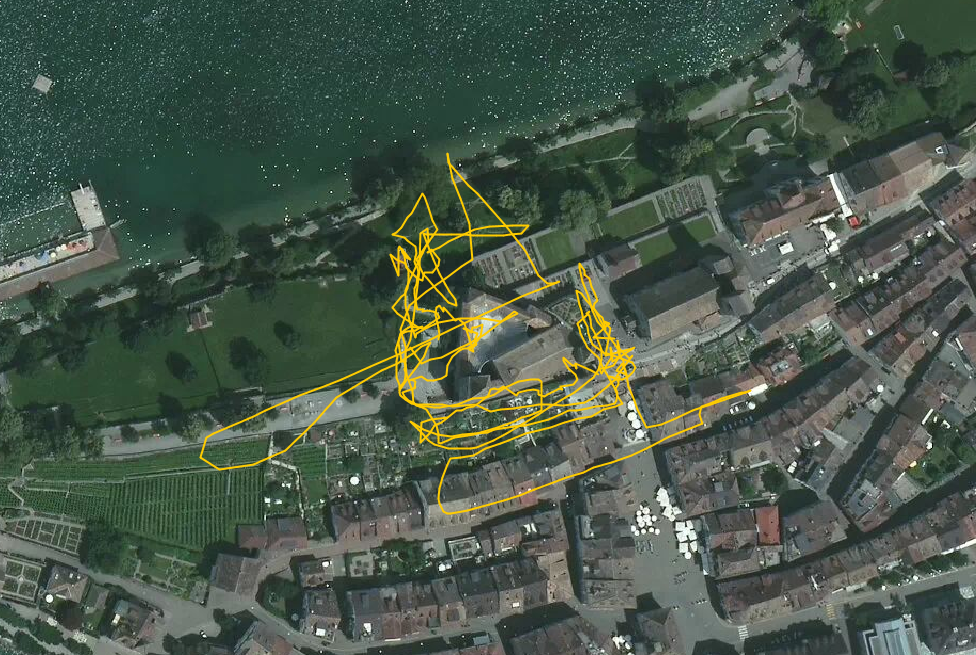
\includegraphics[width=\textwidth]{images/gpstrace_satellite.png}
	\caption{GPS Trace des Quadrokopters während der Erfassung.\\Bildmaterial:
		\copyright{} Bing Maps}
	\label{img:gpstrace-satellite}
\end{figure}

\begin{figure}[p]
	\centering
	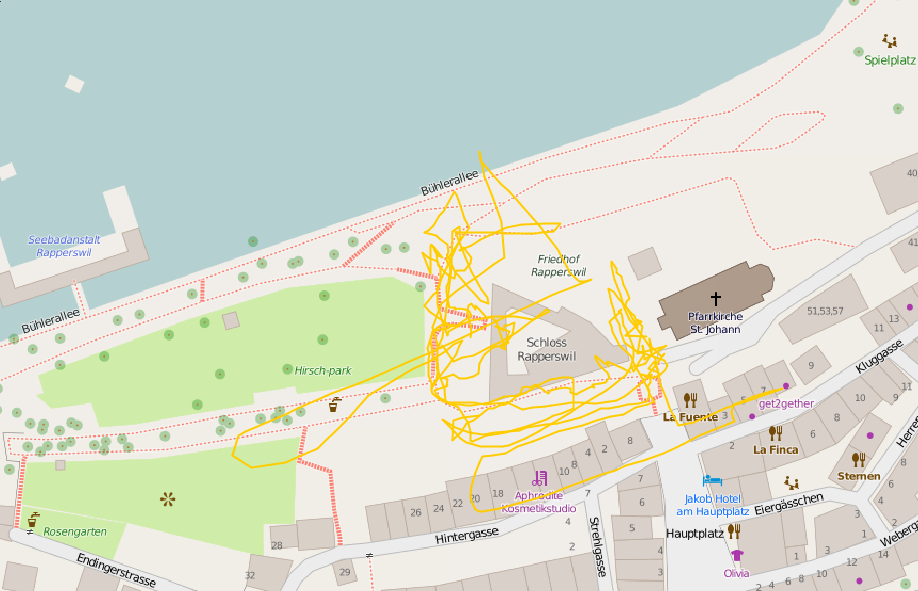
\includegraphics[width=\textwidth]{images/gpstrace_mapnik.png}
	\caption{GPS Trace des Quadrokopters während der Erfassung.\\Bildmaterial:
		\copyright{} OpenStreetMap Contributors}
	\label{img:gpstrace-mapnik}
\end{figure}

\subsection{Bildqualität}

Die GoPro Kamera ist für Sportaktivitäten entwickelt worden und hat daher ein
Weitwinkel-Objektiv ("<Fisheye">) eingebaut. Dies ist bestens geeignet um
beispielsweise beim Skifahren einen guten Überblick zu bewahren, für die
Rekonstruktion ist es aber eher nachteilig.

Ein weiterer Faktor ist die Kompression. Um viele Bilder auf der SD-Karte
speichern zu können, werden die JPEG-Bilder stark komprimiert. Die daraus
entstehenden JPEG-Artefakte können die Feature-Detection stören.

Idealerweise würde man daher zur Erfassung eine Spiegelreflex-Kamera mit
neutralem 35mm Objektiv verwenden und alle Bilder im RAW-Format abspeichern.
Diese können dann mit entsprechender Software ohne verlustbehaftete Kompression
in ein für die Photogrammetrie\-/Software nutzbares Format umgewandelt werden.

In unserem Fall waren wir aber durch die Tragfähigkeit des Quadrokopters
eingeschränkt und haben uns stattdessen dafür entschieden, die Bilder am
Computer mithilfe eines Linsenprofils zu entzerren (TODO Referenz). Inzwischen
gibt es allerdings sogar Photogrammetrie\-/Programme welche die GoPro
Linsenprofile direkt unterstützen. Nichtsdestotrotz gibt es sicher Kameras
welche besser für solche Aufgaben geeignet sind als die GoPro.

\subsection{Learnings}

\begin{itemize}
	\item Die Jahreszeit war an sich gut gewählt, da die Bäume im Winter nicht
		belaubt sind, wodurch die Sicht auf das Schloss nicht eingeschränkt wird.
	\item Nachteilig war jedoch der Schnee auf den Dächern. Er überdeckte die
		Dachziegel und führte so bei der Feature-Erkennung zu schlechteren
		Ergebnissen.
	\item Die GoPro hat eine äusserst starke Verzerrung. 
\end{itemize}


%------------------------------------------------

\part{Software-Evaluation}

%\include{chapters/6}
%\include{chapters/7}

%----------------------------------------------------------------------------------------
%	THESIS CONTENT - APPENDICES
%----------------------------------------------------------------------------------------

\appendix

\part{Appendix} % New part of the thesis for the appendix

\chapter{Appendix B -- Installation VisualSFM}

\label{ch:installing-vsfm}

%----------------------------------------------------------------------------------------

Die folgende Anleitung beschreibt die Installation von
VisualSFM\footnote{\url{http://ccwu.me/vsfm/}} (nachfolgend VSFM genannt) auf
einem Computer mit Ubuntu\footnote{\url{http://www.ubuntu.com}} 14.04
Betriebssystem und einer CUDA-fähigen nVidia-Grafikkarte. CUDA-Unterstützung ist
optional, aber empfohlen.

%----------------------------------------------------------------------------------------

\section{Einleitung}

VSFM ist eine GUI-Applikation für 3D-Rekonstruktion mittels "<Structure from
Motion"> (SFM) Technik. Das Projekt integriert viele Einzelkomponenten, die
meist von Universitäten entwickelt wurden. Mehr dazu findet sich im
\autoref{workflow:vsfm}.

\subsection{Abhängigkeiten}

Für den VSFM 3D-Reconstruction Prozess werden folgende Bibliotheken benötigt:

\begin{itemize}
	\item SiftGPU\footnote{\url{http://www.cs.unc.edu/~ccwu/siftgpu/}}:
		Eine SIFT\cite{lowe:2004}-Implementation für GPUs.
	\item PMVS (Patch-based Multi-view Stereo)\footnote{\url{http://www.di.ens.fr/pmvs/}}:
		Erstellung einer Point-Cloud aus Kamerabildern.
		Das Resultat enthält gemeinsame Features als
		Punkte mit an der Kamera ausgerichteten Normalen.
	\item CMVS (Clustering Views for Multi-view Stereo)\footnote{\url{http://www.di.ens.fr/cmvs/}}:
		Ergänzt PMVS um Clustering für schnellere Resultate.
	\item PBA\footnote{\url{http://grail.cs.washington.edu/projects/mcba/}}:
		Bündelblockausgleichung (Englisch: Bundle Adjustment) auf mehreren CPUs.
\end{itemize}

\noindent Da für die meisten dieser Komponenten nicht als Ubuntu-Pakete
verfügbar sind, müssen sie manuell kompiliert werden.

\subsection{Alternativen}

VSFM arbeitet mit vielen alternativen SFM-Programmen zusammen oder kann Teile davon selbst
benutzen. Sie sind jedoch nicht direkt für den Betrieb von VSFM nötig und wurden
nicht näher betrachtet:

\begin{itemize}
	\item CMP-MVS\footnote{\url{http://ptak.felk.cvut.cz/sfmservice/websfm.pl?menu=cmpmvs}}
	\item MVE\footnote{\url{http://www.gris.informatik.tu-darmstadt.de/projects/multiview-environment/}}
	\item SURE\footnote{\url{http://www.ifp.uni-stuttgart.de/publications/software/sure/index.en.html}}
	\item MeshRecon\footnote{\url{http://www-scf.usc.edu/~zkang/software.html}}
\end{itemize}

%----------------------------------------------------------------------------------------

\section{Installation}

Das folgenden Installationsscript bietet eine Hilfe um VSFM auf einem Ubuntu
14.04 System zu installieren.

Im Script werden alle Abhängigkeiten automatisch aus dem Internet
heruntergeladen. Sie sind jedoch ebenfalls auf unserem Fileserver
(\autoref{fileserver}) vorhanden, für den Fall dass die Ressourcen nicht mehr
online verfügbar sind. Es wird empfohlen nicht das ganze Script auf einmal
auszuführen, sondern es Schritt für Schritt durchzugehen. Möglicherweise haben
sich Systemvoraussetzungen in der Zwischenzeit geändert (z.B. nVidia-Treiber).

\begin{minted}[bgcolor=tango-bg,frame=lines,framesep=2mm,samepage=true,fontsize=\footnotesize]{bash} 
# Whole 2D to 3D reconstruction toolchain setup for Ubuntu 14.04 64bit.
# Make sure to enable the multiverse repository!
# Sources: 
# - http://ccwu.me/vsfm/install.html#linux
# - http://www.10flow.com/2012/08/15/
# - http://www.di.ens.fr/cmvs/

# update the system
sudo apt-get update && sudo apt-get upgrade
sudo apt-get install build-essential

# install a proprietary nvidia driver
sudo apt-get install nvidia-331-updates

# prepare dependencies of vsfm, siftgpu, mulicore_bundle_adjustment, 
#                         pmvs-2, cmvs, graclus
sudo apt-get install libgl-dev libglu-dev libx11-dev \
                     libgtk2.0-dev libglew-dev glew-utils libdevil-dev \
                     libboost-all-dev libatlas-cpp-0.6-dev libatlas-dev \
                     imagemagick libatlas3gf-base libcminpack-dev \
                     libgfortran3 libmetis-edf-dev libparmetis-dev \
                     freeglut3-dev libgsl0-dev
sudo apt-get install unzip
sudo apt-get install nvidia-cuda-toolkit

# compile vsfm (framework for 3d reconstruction from motion)
wget http://ccwu.me/vsfm/download/VisualSFM_linux_64bit.zip
unzip VisualSFM_linux_64bit.zip
cd vsfm
make 
cd ..

# compile SiftGPU (feature detection with GPU)
wget -O SiftGPU.zip http://wwwx.cs.unc.edu/~ccwu/cgi-bin/siftgpu.cgi
unzip SiftGPU.zip
cd SiftGPU
sudo ln -s /usr/lib/nvidia-cuda-toolkit /usr/local/cuda
make
cd ..
cp SiftGPU/bin/libsiftgpu.so vsfm/bin/

# pba (fast bundle adjustments library)
wget http://grail.cs.washington.edu/projects/mcba/pba_v1.0.5.zip 
unzip pba_v1.0.5.zip
cd pba
sed -i.bak 's|CUDA_INSTALL_PATH = /usr/local/cuda|CUDA_INSTALL_PATH \
           = /usr/lib/nvidia-cuda-toolkit|g' ./makefile
make
cd ..
cp pba/bin/libpba.so vsfm/bin/

# pmvs-2 (builds a point cloud of features seen in multiple views)
sudo apt-get install liblapack-dev
wget http://www.di.ens.fr/pmvs/pmvs-2-fix0.tar.gz
tar xf pmvs-2-fix0.tar.gz
cd pmvs-2/program/main/
make clean

wget http://www.10flow.com/wp-content/uploads/2012/08/mylapack.o.tar.gz
tar xf mylapack.o.tar.gz
make depend
make
cd ../../../
\end{minted}

\begin{minted}[bgcolor=tango-bg,frame=lines,framesep=2mm,samepage=true,fontsize=\footnotesize]{bash} 
# graclus (fast graph clustering library)
wget http://www.cs.utexas.edu/users/dml/Software/graclus1.2.tar.gz
tar xf graclus1.2.tar.gz
cd graclus1.2/
sed -i.bak 's|COPTIONS = -DNUMBITS=32|COPTIONS \
           = -DNUMBITS=64|g' Makefile.in
make
cd ..

# cmvs (cluster pmvs output)
wget http://www.di.ens.fr/cmvs/cmvs-fix2.tar.gz
tar xf cmvs-fix2.tar.gz
cp pmvs-2/program/main/mylapack.o cmvs/program/main/
sed -i.bak '1s/^/#include <vector>\n#include <numeric>\n/' \
           cmvs/program/base/cmvs/bundle.cc
sed -i.bak '1s/^/#include <stdlib.h>\n/' cmvs/program/main/genOption.cc
sed -i.bak 's|YOUR_INCLUDE_METIS_PATH =|YOUR_INCLUDE_METIS_PATH \
           = -I'$(pwd)'/graclus1.2/metisLib|g' \
           cmvs/program/main/Makefile
sed -i.bak 's|YOUR_LDLIB_PATH =|YOUR_LDLIB_PATH \
           = -L'$(pwd)'/graclus1.2|g' cmvs/program/main/Makefile
sed -i.bak 's/^Your\ /# Your /g' cmvs/program/main/Makefile
cd cmvs/program/main
make

cp cmvs ../../../vsfm/bin
cp pmvs2 ../../../vsfm/bin
cp genOption ../../../vsfm/bin

# set export paths
echo "" >> ~/.bashrc
echo export PATH=\$PATH:$(pwd)/vsfm/bin >> ~/.bashrc
echo export LD_LIBRARY_PATH=\$LD_LIBRARY_PATH:$(pwd)/vsfm/bin \
            >> ~/.bashrc
\end{minted}




%\include{chapters/0B} % Appendix B - empty template

%----------------------------------------------------------------------------------------
%	POST-CONTENT THESIS PAGES
%----------------------------------------------------------------------------------------

\cleardoublepage% Bibliography

\label{app:bibliography} % Reference the bibliography elsewhere with \autoref{app:bibliography}

\manualmark
\markboth{\spacedlowsmallcaps{\bibname}}{\spacedlowsmallcaps{\bibname}} 
\refstepcounter{dummy}

\addtocontents{toc}{\protect\vspace{\beforebibskip}} % Place the bibliography slightly below the rest of the document content in the table of contents
\addcontentsline{toc}{chapter}{\tocEntry{\bibname}}

\bibliographystyle{plainnat}

\bibliography{bibliography}
 % Bibliography

%----------------------------------------------------------------------------------------

\end{document}
